% Explore the strategy of varying dialect by observing openvpn
% (1) tightening constraint on edge can remove unwanted or vulnerable component
% (2) preserving constraint on edge can also cause the change to outfacing interface
% (3) relaxing constraint is not a good idea because (1) introducing non-deterministic (2) enlarge attack surface
% (4) Add new states
% (5) Remove states through message removal
% (6) Add State though introducing new messages

% \newpage

\section{Generating Various Dialects}
\label{sec:dialect}

With finite state machines extracted, we now discuss how we plan to customize a
protocol implementation to generate various dialects. Similar to the
organization of the section above, the following discusses the challenge of
dialect generation, our preliminary exploration and the proposed techniques in
turn.


\subsection{Challenges}
\label{sec:task2:challenges}

Dialect generation needs to take as input a protocol implementation, and
generate various dialects. To achieve this, we have to address two major
challenges below.

\begin{wrapfigure}{r}{0.35\textwidth}
  \centering
  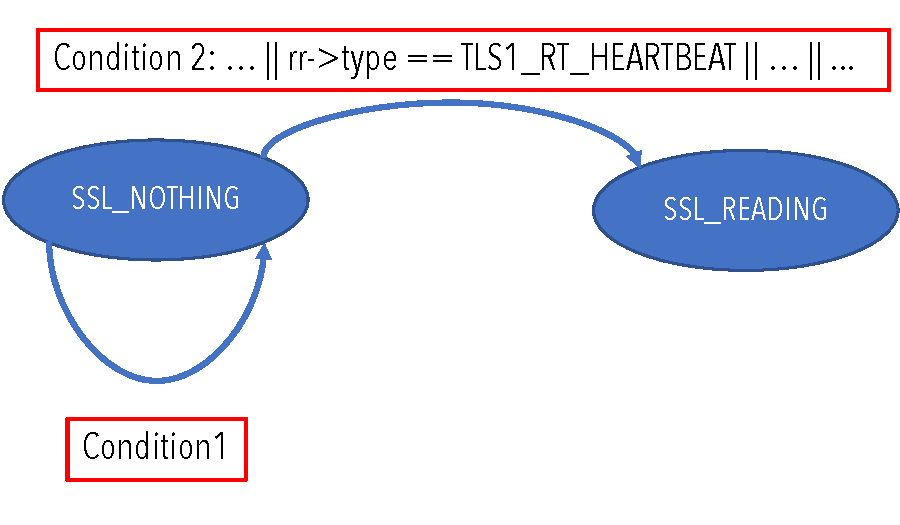
\includegraphics[width=0.3\textwidth]{figure/constraint_tighten}
  \caption{A state machine manually extracted from \texttt{OpenSSL}.}
  \label{fig:tighten}
\end{wrapfigure}

\noindent{\textbf{Validity.}}  To generate a new dialect, there are many
possible approaches. However, many of them may not guarantee the reliability (or
validity) of a dialect newly generated (\eg, generating a new dialect for
\texttt{TCP} communication by eliminating the three-way handshake). As a result,
the first challenge of dialect generation is to identify a set of effective
strategies that can generate new protocol dialects but not introduce
incorrectness.

\noindent{\textbf{Consistency.}} A communication protocol typically involves
more than one parties exchanging messages between each other. Typically, an
implementation pertaining to such a protocol are separated into different code
bases and even involved in multiple parties. When generating new dialects, we
must perform program analysis and modify a protocol implementation across
different code bases. However, research in the past mostly focuses on performing
program analysis on a single code base. Therefore, our second challenge is to
develop a set of effective techniques to perform program analysis across
different code bases and thus ensure the consistency in code variation.


\subsection{Preliminary Exploration}
\label{sec:task2:obs}

Our preliminary exploration lies in a manual study with the goal of identifying
the strategies capable of generating new and more importantly valid protocol
dialects. In the following, we describe the strategies we studied and pinpoint
those that we will use for dialect generation.

\subsubsection{Customizing Dialect with Transition Condition Variation}

Since a protocol dialect typically relies upon finite state machines, our study
first focuses on exploring how to generate new valid dialects by varying state
transitions. To be specific, we manually studied three strategies to vary
transition conditions.


\begin{wraptable}{r}{.38\textwidth}
\centering
\begin{tabular}{c}
\hspace{12pt}

\begin{lstlisting}  
else if (rr->type == TLS1_RT_HEARTBEAT) {
  dtls1_process_heartbeat(s); /* Vulnerable function */
  rr->length = 0;
  s->rwstate=SSL_READING;
  BIO_clear_retry_flags(SSL_get_rbio(s));
  BIO_set_retry_read(SSL_get_rbio(s));
  return(-1);
}
\end{lstlisting}

\end{tabular}
\caption{A code snippet under the condition eliminated vulnerable to the 
heartbleed bug.}
\label{code:heartbleed}
\end{wraptable} 

\noindent{\textbf{Tightening transition conditions}} is a strategy where we
eliminate  some conditions to tighten the constraint of triggering a state
transition. To illustrate this, we take for example the state machine manually
extracted from \texttt{OpenSSL} (see Figure~\ref{fig:tighten}). By removing
condition \Code{rr->type == TLS1_RT_HEARTBEAT} on the state machine as well as
the corresponding implementation in source code, we could tighten the condition
pertaining to the transition from state \texttt{SSL\_NOTHING} to
\texttt{SSL\_READING}, and cut off the code pertaining to the condition
eliminated. In this example, the code of removal includes the heartbeat
component vulnerable to the heartbleed bug~\citep{}, responsible for sending
heartbeat messages between the client and server (see
Table~\ref{code:heartbleed}). Therefore, we could obtain a new dialect without
the heartbeat messages. Since the heartbeat messages are optional for
\texttt{OpenSSL}, we believe this strategy is valid for generating new dialects.
In this project, we will take this condition tightening as \emph{the first
strategy} for generating new dialects.

\begin{wrapfigure}{r}{0.35\textwidth}
  \centering
  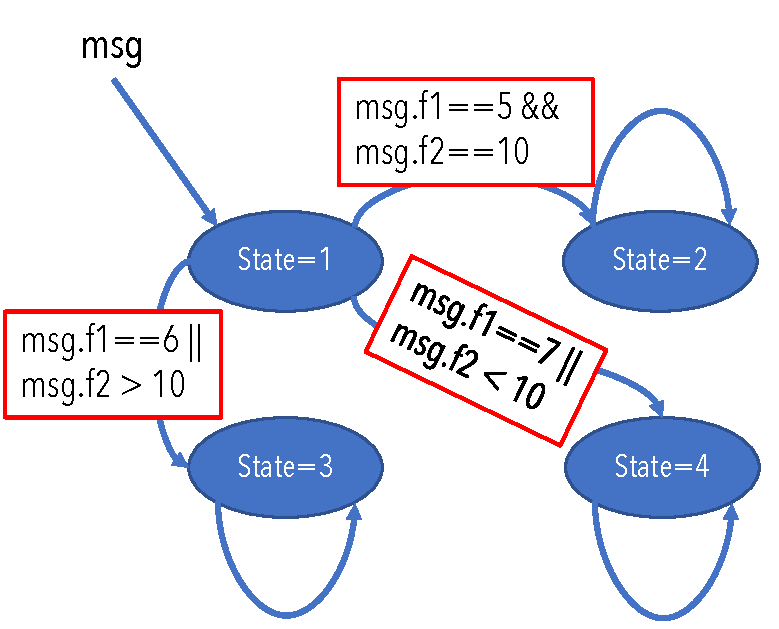
\includegraphics[width=0.3\textwidth]{figure/toy}
  \caption{A toy state machine taking as input message \texttt{msg} from a
  client side. Note that the constraints in the text boxes indicate transition
  conditions, and the message carries integer data in two fields --
  \texttt{msg.f1} and \texttt{msg.f2}.}
  \label{fig:toy_fsm}
\end{wrapfigure}

\noindent{\textbf{Relaxing transition conditions}} is another strategy,  in
which we get rid of a condition to relax the constraint of triggering a state
transition. To illustrate this, we take for example a toy protocol, a finite
state machine of which is shown in Figure~\ref{fig:toy_fsm}. By getting rid of
condition \Code{msg.f2==10}, we can relax the constraint pertaining to the
transition from state \texttt{1} to state \texttt{2}. It is not difficult to
note that such a mutation practice introduces non-deterministic to the state
machine newly generated, especially when the input message holds condition
\Code{msg.f1==5 && msg.f2 > 10}. As a result, we believe this transition
mutation is not suitable for generating a new dialect. In this project, we will
avoid performing dialect generation by following this strategy.

\begin{figure*}
  \centering
  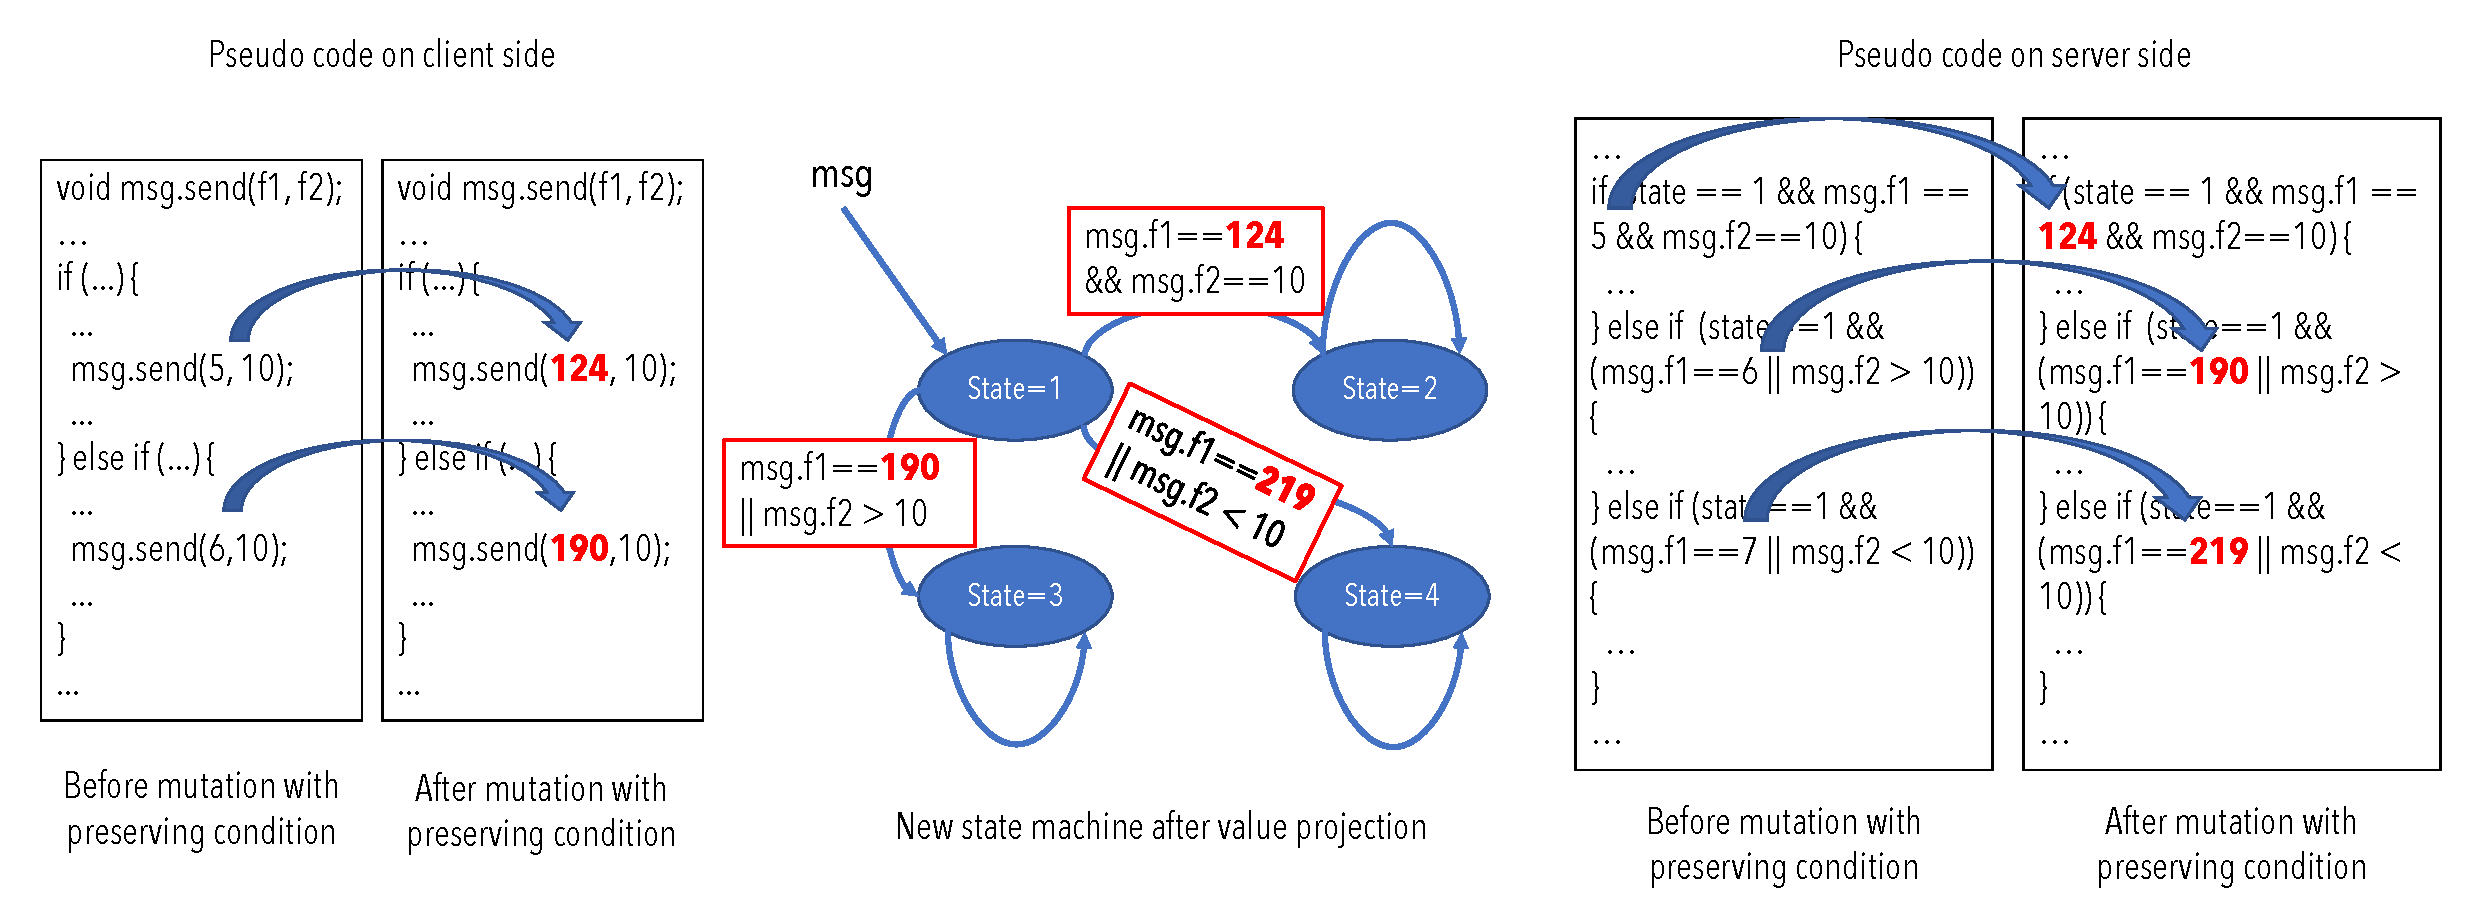
\includegraphics[width=0.95\textwidth]{figure/shuffle}
  \caption{The new state machine and pseudo code generated by following the
  strategy of preserving transition conditions.}
  \vspace{-0.1in} 
  \label{fig:toy_shuffle}
\end{figure*}

\noindent{\textbf{Preserving transition conditions}} is a strategy  where we
vary individual transition conditions and at the same time preserve the one
indicating their combination. To illustrate this, we again take for example the
state machine shown in Figure~\ref{fig:toy_fsm}. Assume \texttt{msg.f1} in
condition \Code{msg.f1==5 && msg.f2==10} is an integer variable with the values
from 5 to 7, indicating the operation code received from a client side. By
projecting these three values into new value space \texttt{(124, 190, 219)} and modifying the
corresponding implementation on both ends (see Figure~\ref{fig:toy_shuffle}), we
can change the state machine to a new one -- with the only difference in the
state transitions -- and thus generate a new dialect in which both the client
and server use new messages to coordinate the state transition. In this project,
we will take this as \emph{the second strategy} for customizing protocol
dialects.

\subsubsection{Customizing Dialect with State Variation}

To identify effective strategies for dialect generation, we also investigate how
to generate a new valid dialect by varying the transition states pertaining to
state machines extracted from a target protocol. Technically speaking, there are
many strategies to mutate transition states and vary dialects, such as deleting
and adding states. However, some practices clearly do not guarantee the
correctness of dialects newly generated. Take \texttt{OpenVPN} for example.
Figure~\ref{fig:original_dialect} illustrates a dialect of \texttt{OpenVPN} in
which the first three messages indicate a three-way handshake. By simply
removing state \texttt{S\_PRE\_START}, which further results in the elimination
of the message attached (\texttt{P\_ACK}), we can easily break the semantic of
this protocol, making message transmission unreliable. As a result, we will
avoid adding or deleting transition states in an arbitrary manner. In our
preliminary study, we have identified two strategies to perform reliable state
addition and removal. Here, we summarize both below.

\begin{wrapfigure}{r}{0.35\textwidth}
  \centering
  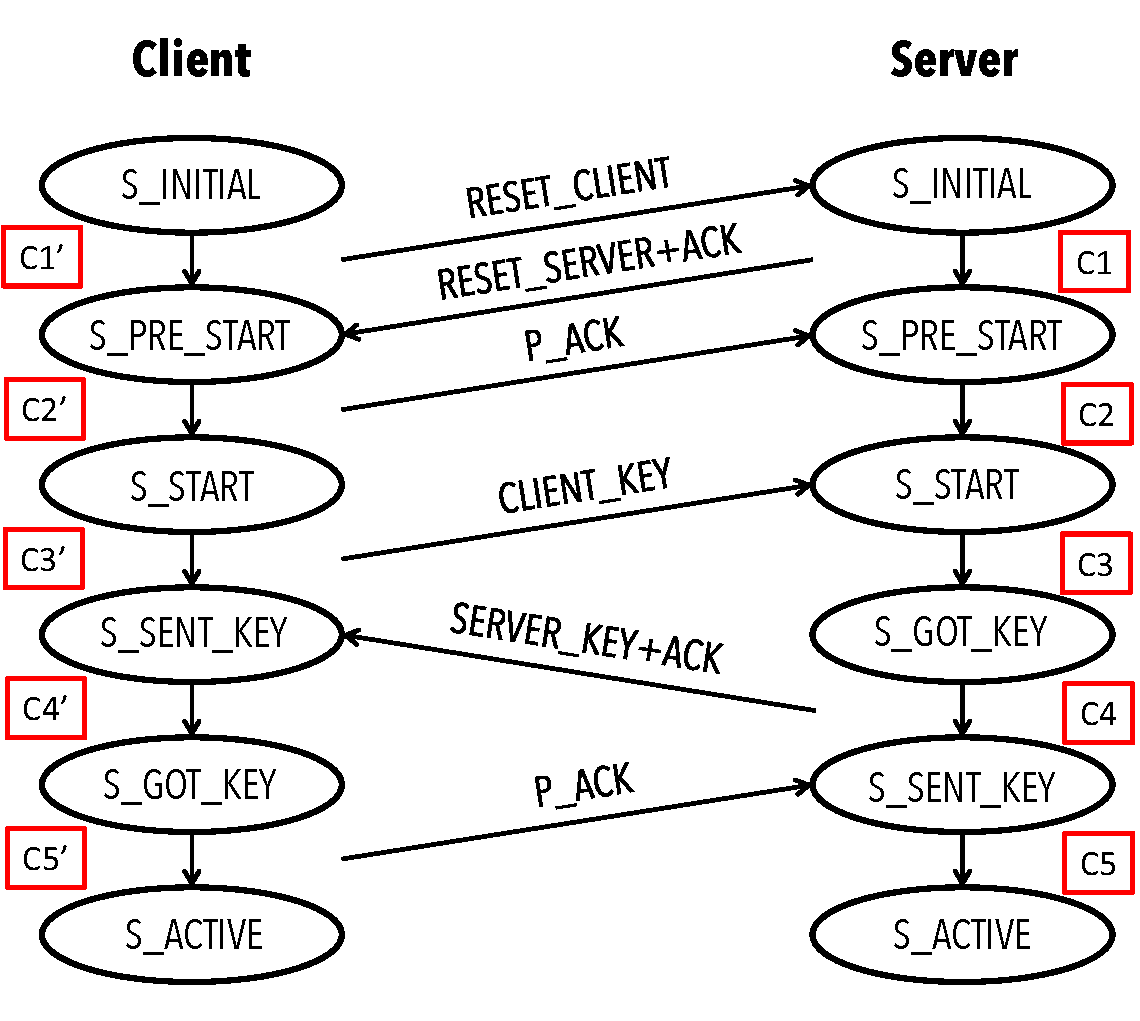
\includegraphics[width=0.3\textwidth]{figure/dialect}
  \caption{One dialect implemented in \texttt{OpenVPN} responsible for
  establishing a private communication tunnel. Note that the ovals indicate
  transition states in finite state machines extracted from \texttt{OpenVPN},
  the edges between them demonstrate the transitions from one state to another
  and the textboxes attached to the edges denote transition conditions.}  
  \label{fig:original_dialect}
\end{wrapfigure}


\begin{figure*}[t]
\centering
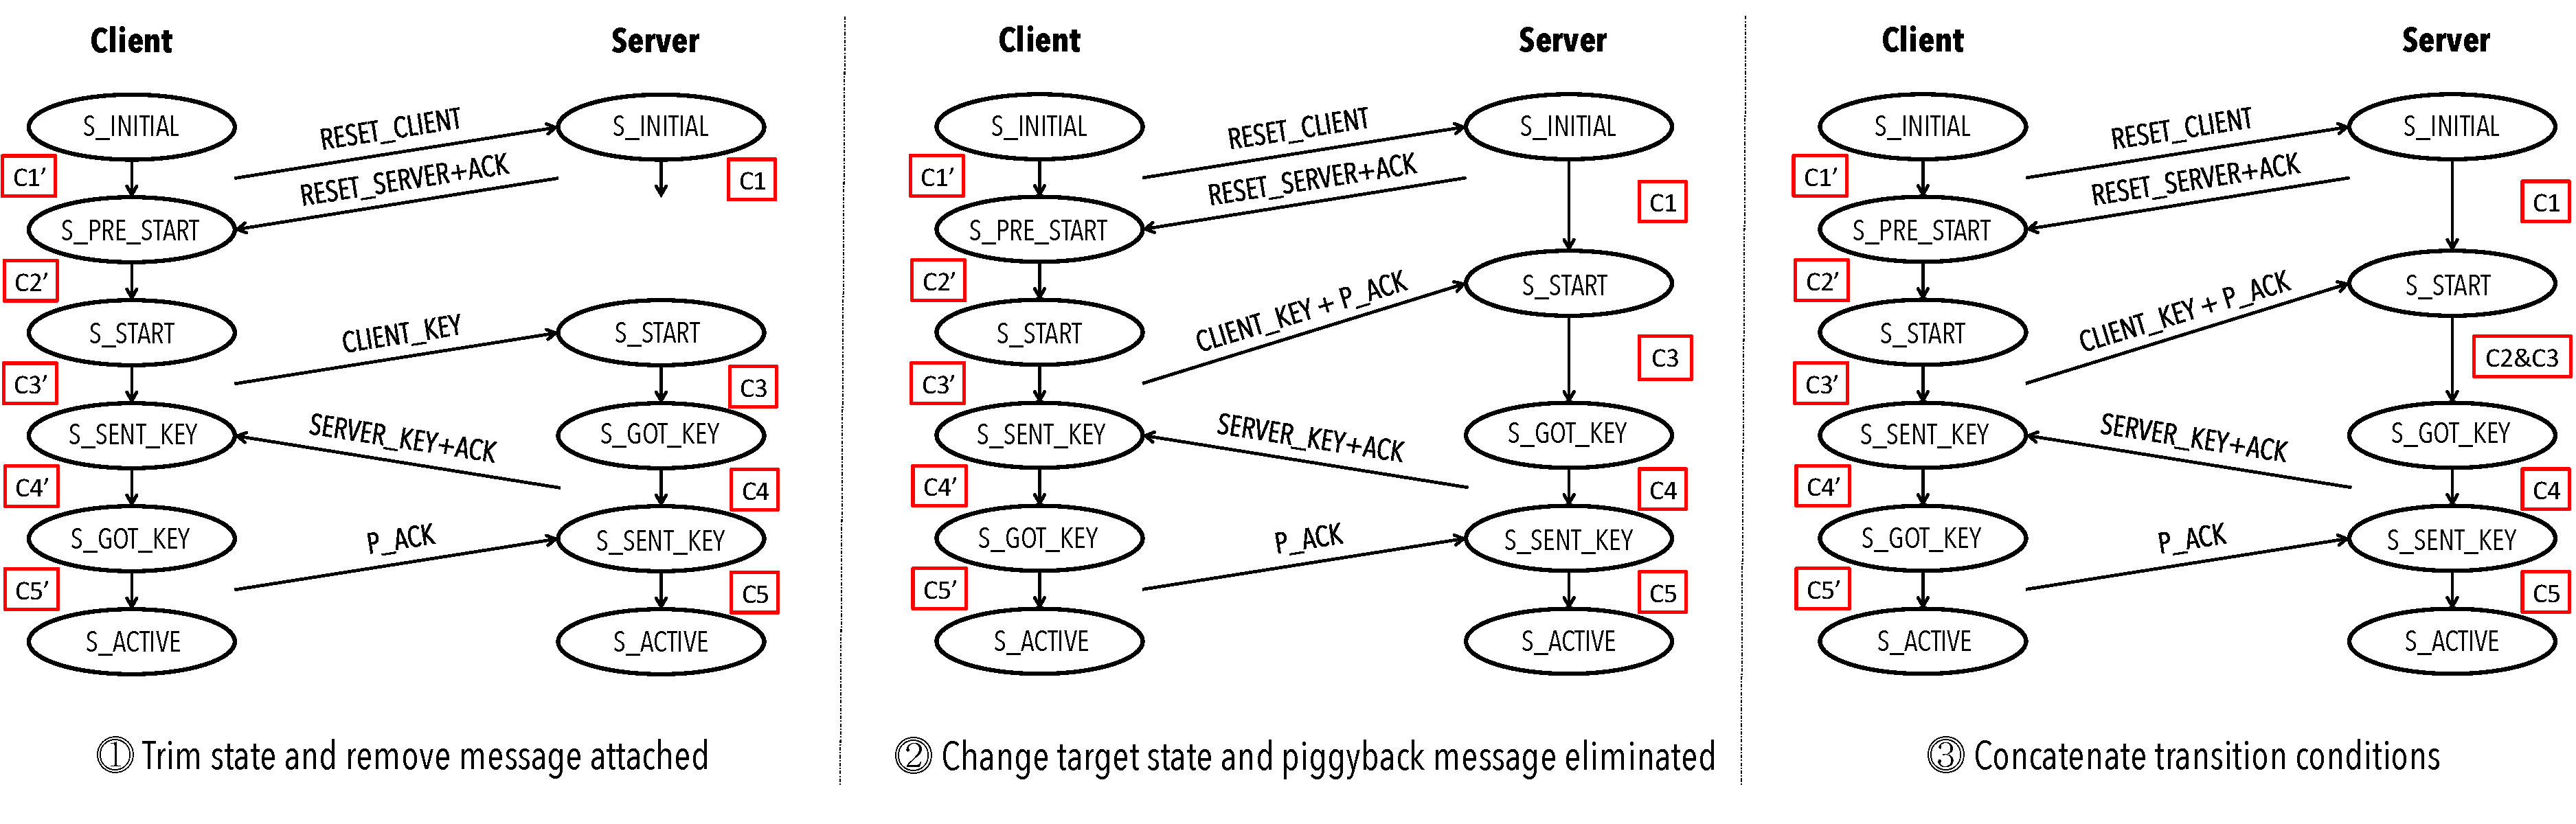
\includegraphics[width=0.95\textwidth]{figure/state_removal}
\caption{The procedure of generating a protocol dialect by removing transition 
states.} 
\vspace{-0.1in} 
\label{fig:state_removal} 
\end{figure*} 

{\noindent{\textbf{Eliminating states with message merging}} is a strategy
where we preserve protocol semantic by removing a state and merging the message
attached with a consecutive message. To illustrate this, we take
\texttt{OpenVPN} for example. As is shown in Figure~\ref{fig:state_removal}, we
first trim transition state \texttt{S\_PRE\_START} and disable the function
responsible for sending message \texttt{P\_ACK}. Second, we change the target
state under condition \texttt{C1} and append the information carried by
\texttt{P\_ACK} to consecutive message \texttt{CLIENT\_KEY}. To be able to check
message \texttt{P\_ACK} piggybacking on \texttt{CLIENT\_KEY}, we finally
concatenate the transition conditions with a logic conjunction operator. In this
way, we preserve the message needed for the 3-way handshake in a consecutive
message. Thus, it guarantees the legitimacy of the new dialect. In this project,
we will take this state elimination as \emph{the third strategy} for our dialect
generation.


\begin{figure*}[t]
\centering
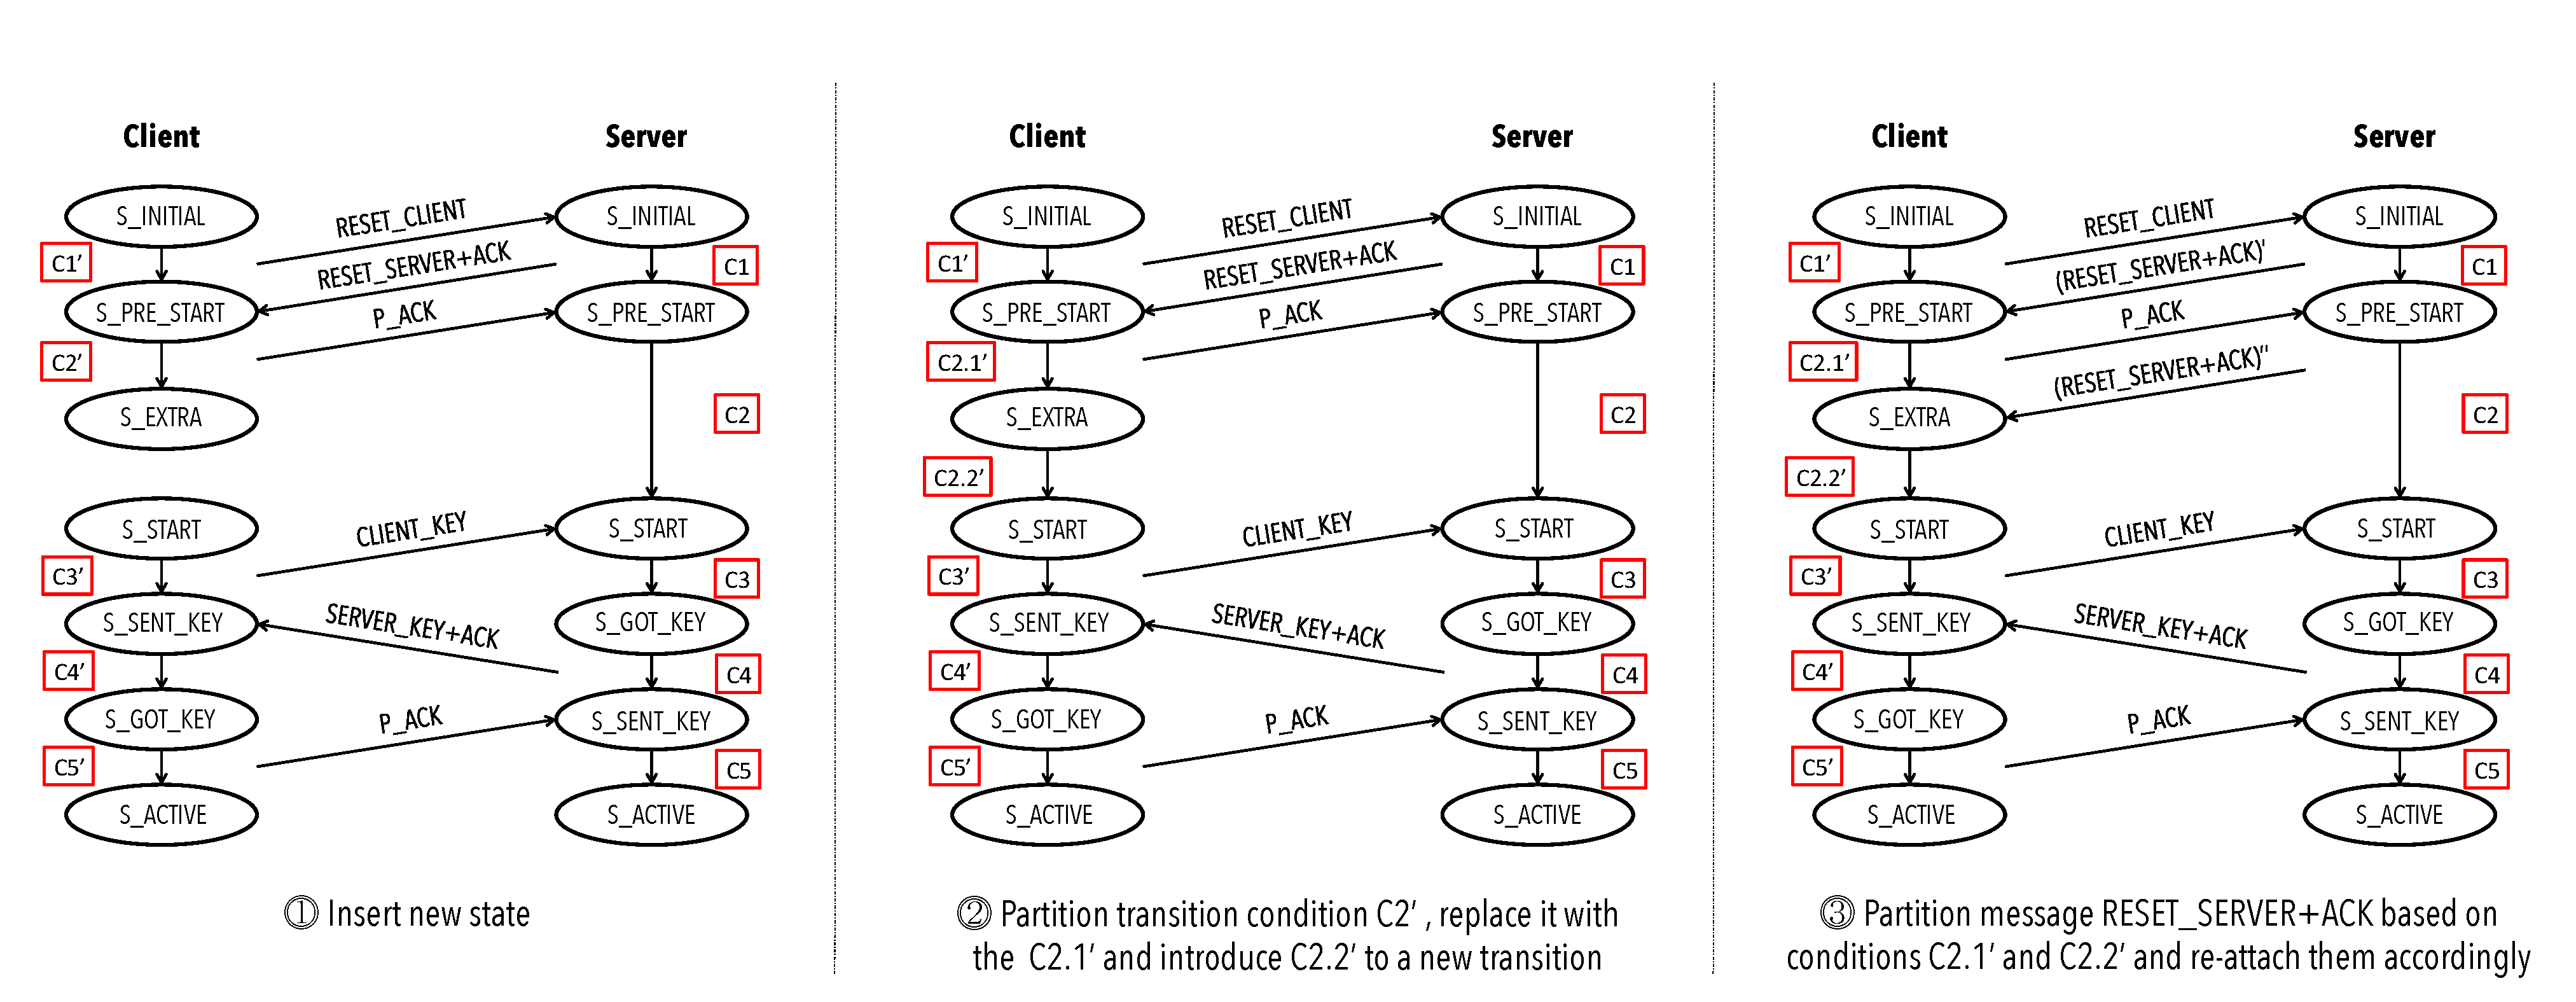
\includegraphics[width=0.95\textwidth]{figure/state_addition}
\caption{The procedure of generating a protocol dialect by introducing a new 
  transition state.} 
\vspace{-0.1in} 
\label{fig:state_addition} 
\end{figure*} 

{\noindent{\textbf{Introducing states with message partition}} is a  strategy in
which we introduce not only a new state but also partition a message. Again, we
take \texttt{OpenVPN} for example. As is shown in the first two diagrams of
Figure~\ref{fig:state_addition}, we first insert additional state
\texttt{EXTRA\_CLIENT} between states \texttt{S\_PRE\_START} and
\texttt{S\_START} by changing the target state under condition \texttt{C2'}.
Second, we partition condition \texttt{C2'} into two individual constraints
\texttt{C2.1'} and \texttt{C2.2'} so that the disjunction of these two is
equivalent to \texttt{C2'} (\ie, \Code{C2.1'||C2.2'=C2'}). Third, we replace
transition condition \texttt{C2'} with \texttt{C2.1'}, and introduce a new
transition from state \texttt{S\_EXTRA} to state \texttt{S\_START} under
condition \texttt{C2.2'}.

Since condition \texttt{C2.1'} is the tightened version of \texttt{C2'}, and
message \texttt{RESET\_SERVER+ACK} is not able to trigger the state transition
from \texttt{S\_PRE\_START} to \texttt{S\_EXTRA}, we further adjust the
implementation based on the condition replaced, and introduce a code snippet
capable of generating a message that can trigger the transition from state
\texttt{S\_EXTRA} to state \texttt{S\_START }. By inserting this code snippet
into the server code base indicating the transition from state
\texttt{S\_PRE\_START} to state \texttt{S\_START}, we construct a new dialect in
which we introduce a new state to receive the partitioned message needed for the
protocol. As we can observe from the last diagram of
Figure~\ref{fig:state_addition}, the dialect newly generated does not discard
any information. Thus, this strategy ensures the  legitimacy of the new dialect.
In this project, we will take this state elimination as \emph{the fourth
strategy} for our dialect generation.

\subsection{Proposed Techniques}

As is mentioned above, the strategies identified for dialect generation involve
code removal (\eg, tightening transition conditions requires the removal of the
code under the eliminated condition) as well as code synthesis (\eg, introducing
new transition states requires the synthesis of the code for sending out the
message partitioned). Therefore, our proposed techniques mainly focus on
designing effective code removal and synthesis mechanisms for the strategies
mentioned above.

\subsubsection{Research Task 4: Enabling Code Removal with Dialect Recovery}

In the context of protocol customization, it is generally challenging to achieve
a clean code removal. Take the condition tightening strategy for example. We can
easily pinpoint the code fragment under the removal condition. However, this is
far from sufficient because the code unnecessary for a new dialect is typically
distributed beyond the site under the condition eliminated. To address this
issue, we will design and develop a mechanism to link all the code fragments to
the one directly presented under the removal condition.

In this project, we plan to enable this mechanism by recovering protocol
dialects. To be specific, we will first identify the finite state machines that
involve communication dialects. Since a communication dialect involves message
exchanging, we intend to achieve this by examining state machines tied to
function calls responsible for message sending and receiving. Second, we will
pair state machines tied to the same dialect. To accomplish this, we plan to
examine the data structure tied to function calls. Here, our hypothesis is that,
if sending and receiving function calls are all tied to the same data structure,
the corresponding state machines are involved to the same dialect. In this
project, we will validate this hypothesis and if needed adjust this technique
based on protocol implementations.

After identifying and pairing state machines, we will then recover the sequence
of the messages exchanged between the state machines paired together. To do
this, we plan to  perform value set analysis on the code base corresponding to
each of the state machines. Similar to the technique proposed for refining a
state machine in Section~\ref{subsec:rt3}, we will conduct this analysis against
the outgoing messages prior to its attachment to message sending, and then match
that value set with transition conditions of the state machine present on the
other side. To illustrate this approach, we take \texttt{OpenVPN} for example.
By performing a value set analysis at a site where a client state machine
sends a request message, we obtain a set of values for the message which
perfectly match transition condition \Code{!(&ks->plaintext_write_buf->len) &&
!session->opt->server && packet.opcode == P_CONTROL_HARD_RESET_CLIENT_V2}
present on the edge of a server state machine.

With a protocol dialect restored, it is not difficult to notice that one could
easily pinpoint the messages exchanged between each other which can be further
used for tracking down the code fragments pertaining to that of removal. For
example, by tightening the transition condition on the server from state
\texttt{S\_PRE\_START} to \texttt{S\_START} illustrated in
Figure~\ref{fig:original_dialect}, we can use the dialect to pinpoint the call
to that function responsible for sending \texttt{P\_ACK}. On the code base
running on the client side, we can then perform backward taint and identify the
code fragments relevant to message \texttt{P\_ACK} holding the removed
condition. In this project, we will use the output of this backward taint to
guide our code fragment removal.


\subsubsection{Research Task 5: Customizing Code Synthesis Mechanisms for 
Dialect Generation Strategies}

Dialect generation strategies represent different ways to modify a protocol
implementation. For example, the first strategy mainly involves code
modification through code removal, whereas the third strategy introduces
implementation variation by adding new code and restructuring code fragments. As
a result, we must  go beyond code removal, and explore other code synthesis
mechanisms. In this project, we plan to design and develop different code
synthesis mechanisms for each of the strategies mentioned above.

For the first strategy, we will first use the aforementioned approach to
identify the code fragment relevant to the condition eliminated. Then, we will
cut off the code fragments identified, and replace the code fragment under the
removal condition with an exception handler. In this project, we will introduce
the exception handler to throw a notification while it is triggered. The reason
is that this could augment the new protocol with the ability to pinpoint the
messages that mismatch the new dialect.

For the second strategy, we will first perform value set analysis for the
variables of interest (\ie, those that we will perform value modification).
Then, we will project the set of values into a new value space. Using the
protocol dialog recovered, we will identify the site where the variables of
interest are defined, and replace the values for the variables accordingly. To
ensure the value replacement does not break the program semantic, we will
further perform a data flow analysis and if needed adjust the source code
accordingly. For example, a protocol implementation may check a condition (\eg,
\Code{if(x+y>16){...}}) which relies upon variable \texttt{x}, the value of
which has been replaced. To ensure program correctness, we need to propagate
this modification to the condition. In this project, we will explore various
approaches to achieve value projection. In addition, we will design effective
mechanisms to propagate value variations and thus achieve code modification in a
correct manner.

For the third strategy, we will first identify the code statement, indicating
the transition from predecessor states to the state of removal. From the site of
each statement identified, we will then perform a backward taint analysis to
identify the function attached to the transition responsible for receiving a
message. Using the dialog we recovered, we will trace back the message we
identified, and pinpoint the site where the function sends out the message that
we would like to piggyback. To prevent the function sending out the message, we
will remove the line of code indicating the call and introduce a buffer to hold
the message. Since the buffer we introduce will be a global variable, we could
still  retrieve the message at the site where we will perform piggybacking. In
this project, we will explore how to encode the message in the buffer into the
corresponding consecutive message.

For the last strategy, we will first extend the value set of the variable
indicating the transition state. Then, we construct an \texttt{if-else} template
based on the partitioned conditions, and perform a forward program slicing
starting from the sites of interest (\ie, the condition of partition as well as
the message we will separate). With the code sliced, we will fill in the
template, and thus synthesize the code fragments pertaining to the new
transitions. In this project, we intend to use these synthesized code fragments
as replacements for the implementation pertaining to the original transitions.


Considering the synthesis mechanisms described above may introduce
incorrectness, as part of the research project, we will also design a static
verification mechanism to identify invalid dialects. To be specific, we will
examine infeasible paths within the implementation of new state machine. By an
infeasible path, we mean a conflicting constraint along an execution path
synthesized. Throughout the project, we will explore how to leverage the output
of this verification mechanism to guide and correct our protocol dialect.





